% !TeX root = ../thesis.tex
\chapter{Introduction} \label{cha:intro}
This thesis covers the development and engineering process of the \gls{EDiC} which is pictured in \cref{fig:EDiCSnake}.
It is a completely novel \gls{CPU} architecture built in order to visualize and demonstrate the fundamental workings of any \gls{CPU}.
The \gls{EDiC} can execute over half a million instructions per second and also features step-by-step debugging as well as breakpoint capabilities to enable a better understanding of how \glspl{CPU} work.
All components can be tested individually with the help of dedicated test adapters and, thus, \gls{IC} failures can be tracked down and fixed easily.
Additionally, to the hardware build, the project includes an open source development environment including an assembler, tools to modify the microcode and also \gls{FPGA} simulation and emulation of the hardware \cite{EDiCGitHub}.
\begin{figure}[t]
  \centering
  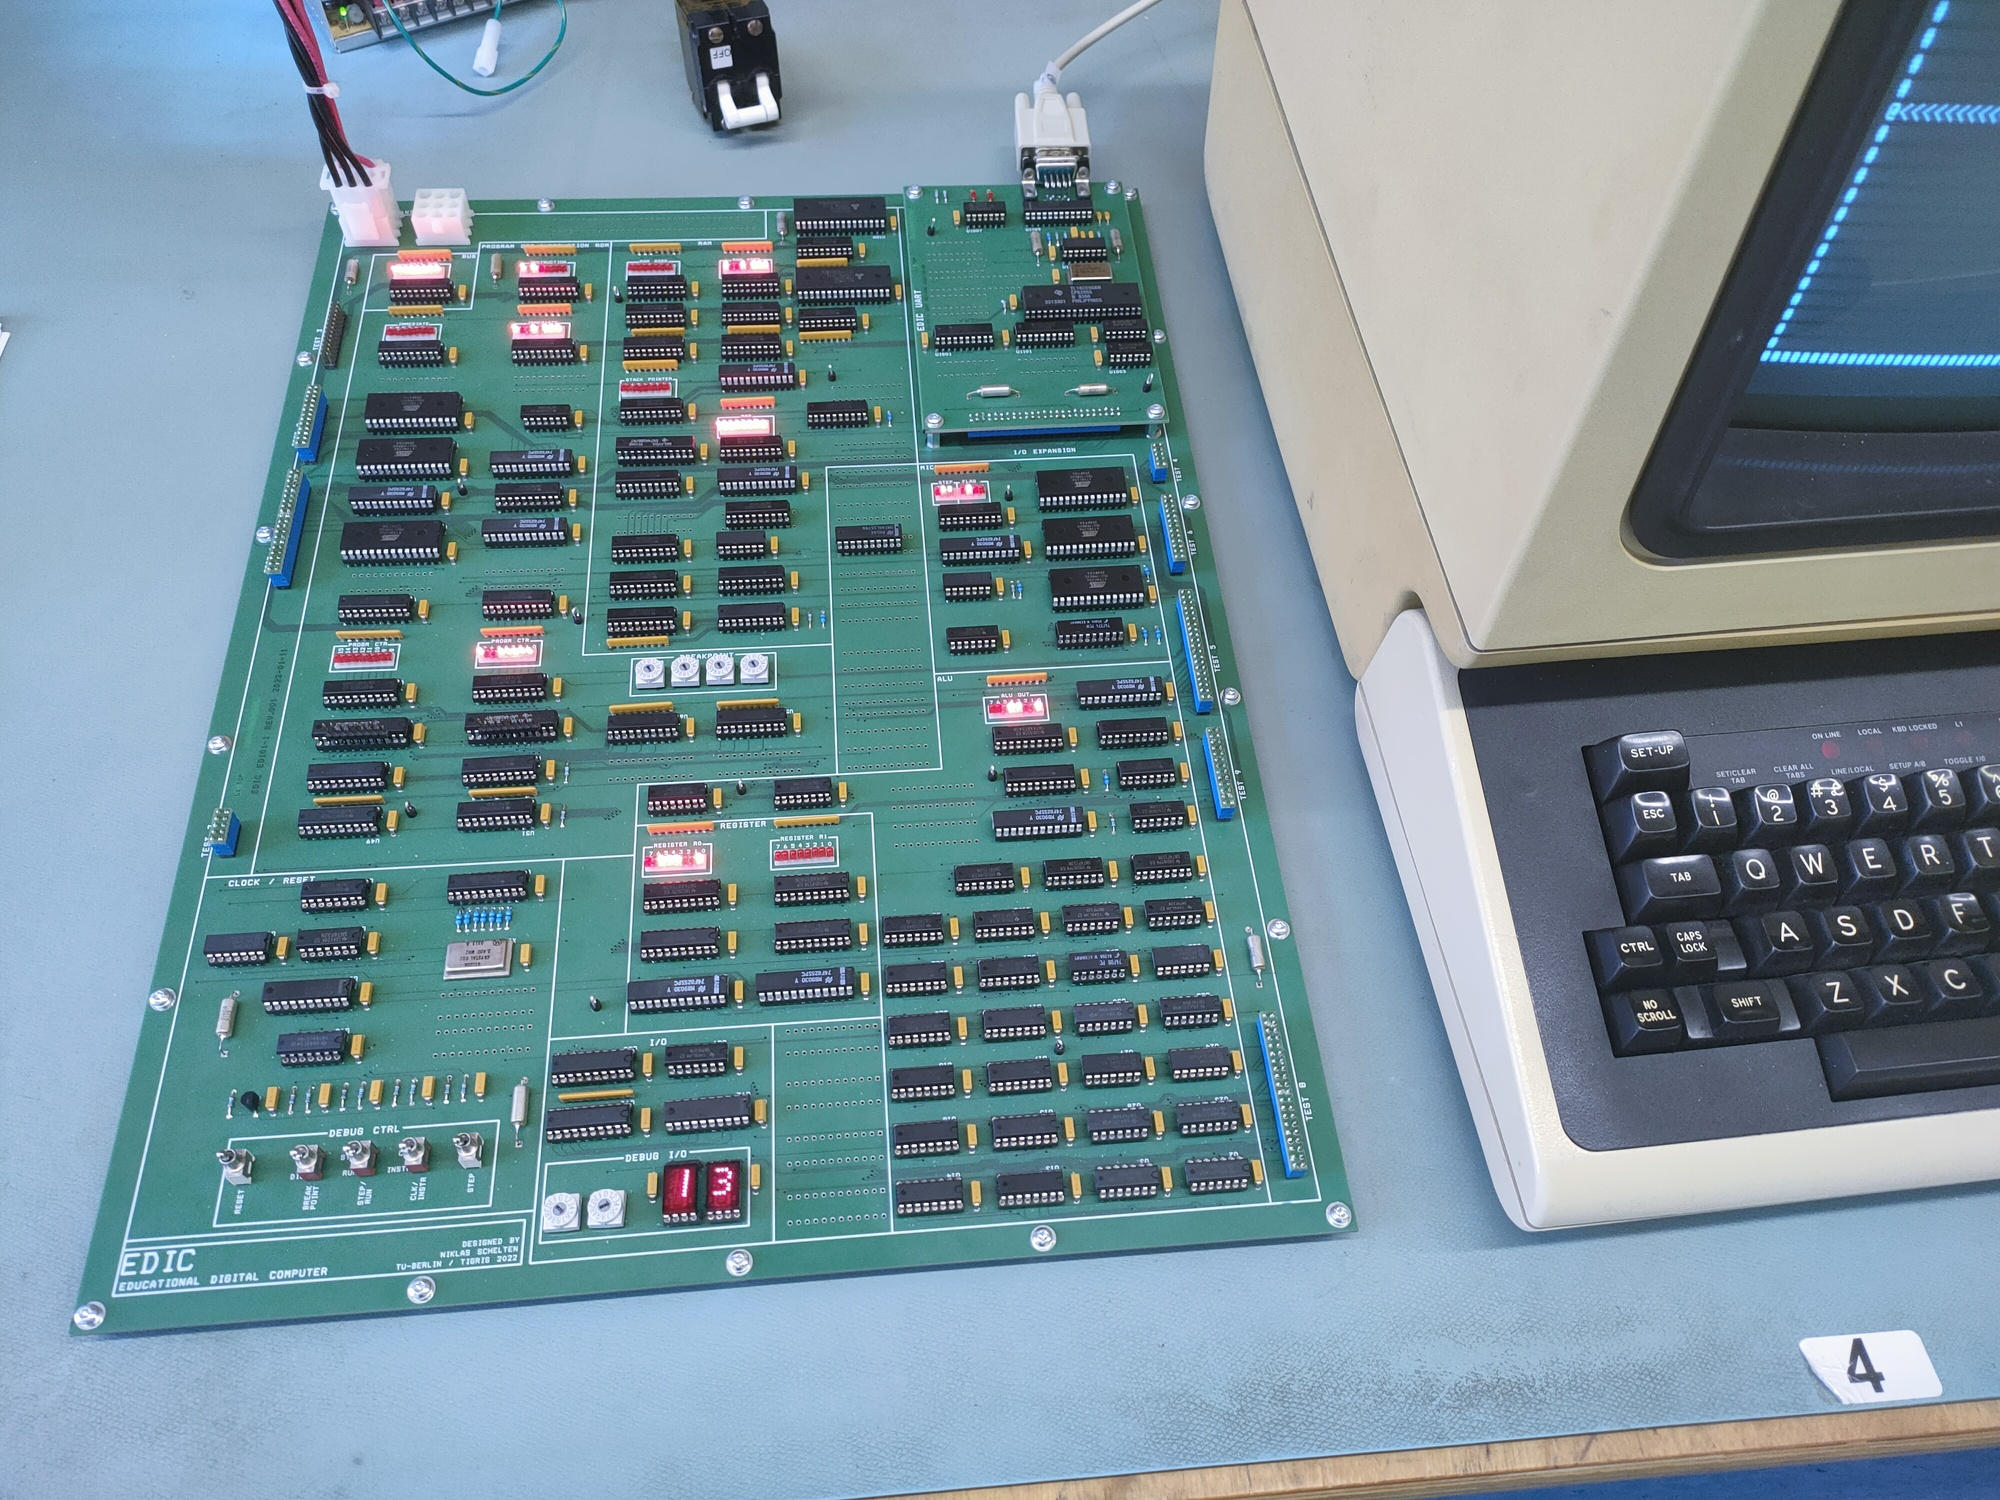
\includegraphics[width=\textwidth]{IMG20220308163628_resize.jpg}
  \caption{The final version of the \gls{EDiC} playing Snake on a VT-100 over an RS-232 I/O card.}
  \label{fig:EDiCSnake}
\end{figure}
\section{Background}
\subsection{Short History on Computing}
The history of computing hardware goes back to ancient times when people used devices like the abacus which simplifies calculations like additions or multiplications.
Starting from the end of the 19th century, analog computers were developed which used continuous physical phenomena to explore complex problems.
One of the first widespread analog computers was created by Sir William Thomson (Lord Kelvin) which predicted tide levels for particular locations by using a set of pulleys and wires. \cite{sep-computing-history}
Even though analog computers could perform very complex operations like solving differential equations \cite{analogDiff} they also had the major drawback that, due to their analog and continues nature, it was not possible to exactly recreate a calculation.

The idea of modern, digital computers was firstly theorized by Alan Turing in his paper \emph{On Computable Numbers} in 1936. \cite{10.1112/plms/s2-42.1.230}
He introduced the notion of a universal (Turing) machine which describes a machine that is provable capable of computing everything that is computable.
All the computers today are as capable as a turing machine which is expressed by calling them \emph{turing complete}.
This is with exception from their finite memory and limited number range.
The first digital computers from the mid 20th century were mechanical or electromechanical machines which combined basic switches like relays and mostly mechanical memory.
As fully electrical computers increased the switching frequencies, a lot of different number formats where emerging:
Opposed to analog computers where one signal, e.g. a voltage, \emph{represents} a value, it now needs to \emph{encode} a value.
In the nowadays common binary system one signal encodes either a 0 or a 1 (for example a low and high voltage) but a lot of different number systems where used like bi-quinary\footnote{Bi-quinary has one quinary signal encoding 0-4 or 5-9 depending on one binary signal encoding a low or high number. This allows two signals to encode a decimal digit similarly to some abacuses.}.

A variety of technologies where developed for fully electric computers like vacuum tubes or transistors.
After using discrete transistors, the advent of \glspl{IC} in the late 50s lead to a rapid acceleration of computer complexity and speed while reducing the power consumption drastically.
The first semiconductor \gls{IC} was invented in 1959 \cite[p. 221]{winston1998media} with its first application being in military and space industries in the early 60s.
The series of \glspl{IC} which is the most relevant to this thesis is the \gls{TTL} 74 series.
It is a successor of one of the first \gls{TTL} \glspl{IC} developed by Texas Instruments in 1964 for military applications: The 5400 series. \cite{ICs}
The 5400 series of \glspl{IC} was specified for a temperature range from \qty{-55}{\celsius} to \qty{+125}{\celsius} and came in a ceramic \gls{SMD} to reach the high temperature range and to be low weight.
Each package included a set of basic logic circuits like four 2-input NAND gates in the 5400N.
In 1966 the first \glspl{IC} of the 74 series were released which had the same functions but with a reduced temperature rating of \qty{0}{\celsius} to \qty{+70}{\celsius} and often came in plastic packaging for commercial applications.
For cost reduction and easier usage, they often came in \gls{DIP} and later on also in plastic packages.
In contrast to previous \gls{RTL}, these \gls{TTL} \glspl{IC} were capable of higher switching frequencies and lower power consumption due to a second transistor driving the high voltage level.
See \cref{sec:ttl} for a more in depth description of the workings of a \gls{TTL} gate.
As the 74 family of \glspl{IC} became larger with more complex \glspl{IC}, more advanced technologies, such as \gls{CMOS}, were also introduced into the family to further reduce the power consumption or increase the switching speeds.

With further advances in the complexity and integration of computing nodes, the first microprocessors were developed in the 70s with the famous Intel 4004 and 8080 in 1971 and 1974, respectively.
These processors combine all the logic required for a general purpose \gls{CPU} into one \gls{IC} usually exposing interfaces for connecting memories and user \gls{IO} logic.

\subsection{Technology Selection for the \gls{EDiC}}
The design goal for the \gls{EDiC} was to create a \gls{CPU} which aids the teaching of how \glspl{CPU} generally work.
To build a custom \gls{CPU}, many of the above-mentioned technologies were used for computer design, however, not all of them are equally suited for a model \gls{CPU}.
It was decided to use \gls{TTL} \glspl{IC} of the 74 family in the \gls{EDiC} for several reasons:
\begin{itemize}
  \item \emph{Complexity:} The \glspl{IC} of this family are complex enough to make it possible to build complex systems as a general-purpose \gls{CPU} with only about 100 chips.
  On the other hand, each individual \gls{IC} is easy to understand since it is kept quite simple, for example the 7400 has a basic interface of 12 pins for the four 2-input NAND gates plus GND and +5V pins.

  \item \emph{Speed:} In contrast to previous technologies such as electromechanical relays or \gls{RTL}, the 74 series is a lot faster, particularly the 74F subseries which is mainly used in the \gls{EDiC}.
  It is feasible to create complex designs with the 74F series with a clock frequency of several \unit{\mega\hertz}.
  However, at the same time, the clock frequency is not too high, so that special care must be taken when designing the \gls{PCB} which would be the case with higher frequency signals.

  \item \emph{Simplicity:} Working with the \glspl{IC} is fairly easy: No special tools -- except a soldering iron and oscilloscope -- are required to assemble and test the system.
  Especially the usage of sockets for the \glspl{DIP} simplifies the build because no \gls{IC} can overheat while soldering and all the \glspl{IC} can be replaced later on or while testing.
\end{itemize}

In contrast to previous and also later technology, the \gls{TTL} also stands out as the best suited one.
When trying to build a \gls{CPU} out of discrete transistors, not only the logical level needs to be respected but a lot of static and dynamic behavior of the transistors needs to be analyzed.
This complicates the design and prevents students from comprehending the \gls{CPU} on its logical level.
On the other side, more modern technologies became so abstract and complex to use that the comprehension of the internal workings of the \gls{CPU} could also be lost.
For example, when choosing \glspl{FPGA} as the driving technology, the work surrounding the technology quickly becomes more complex than the \gls{CPU} itself.
The \gls{FPGA} \glspl{IC} require special voltage levels and special care with the high frequency clock traces, are hard to solder with small pins, require complex build toolchains, cannot be debugged with an oscilloscope and so on.

Thus, the \gls{TTL} was the ideal technology level for creating a model \gls{CPU} which helps students understanding the workings of \glspl{CPU}.

\subsection{Workings of \gls{TTL}}\label{sec:ttl}
\begin{figure}[t]
  \centering
  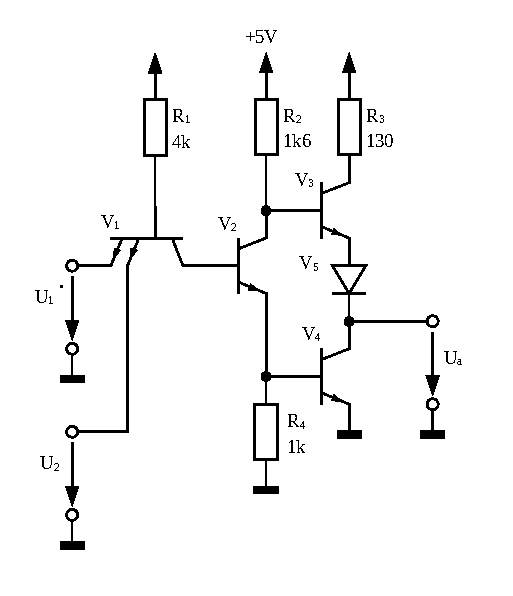
\includegraphics[width=\textwidth]{7400_Circuit.pdf}
  \caption{\gls{TTL} NAND with ``totem-pole'' output stage as in the 7400 \gls{IC}. \cite{7400_Circuit}}
  \label{fig:7400_Circuit}
\end{figure}

\Cref{fig:7400_Circuit} shows the internals of one of the four NAND gates inside the 7400 \gls{IC}.
The multi-emitter transistor $V_1$ functions as the logical NAND gate while the transistors $V_2$, $V_3$ and $V_4$ in combination with the diode $V_5$ form the ``totem-pole'' output stage.
If both inputs are high, a small collector current is drawn by both inputs because $V_1$ is in reverse-active mode.
The current through $R_1$ ``activates'' $V_2$ which in turn ``activates'' $V_4$ due to the current steering effect, where the current flows through the one parallel voltage-stable element with the lowest threshold voltage.
In this case, the current flows through $R_2$, $V_2$ collector-emitter and $V_4$ base-emitter rather than through $V_3$ collector-emitter, $V_5$ and $V_4$ collector-emitter.
Therefore, $V_4$ drives the output with a low voltage.

If one of the inputs is low, on the other hand, the current steering effect turns off $V_2$ since the current flows through $R_1$ and $V_1$ base-emitter rather than $R_1$, $V_1$ base-collector $V_2$ base-emitter and $R_4$.
Hence, the above-mentioned current steering effect on the output stage no longer takes effect and $V_3$ drives the output high through the diode $V_5$.

The advantage of this ``totem-pole'' output stage in comparison to a more simple output stage with the collector of $V_2$ effectively being the output is, that a very low output resistance can be achieved (only the small $R_3$) which allows the output to drive more inputs of other logic gates.
Additionally, the speed is drastically increased because the high output is actively driven instead of pulled up via a resistor as in \gls{RTL}.
However, the voltage drop over $V_3$ and $V_5$ also have the effect that the high output voltage is only about \qty{3.5}{\volt} in contrast to the simpler approach where almost \qty{5}{\volt} can be achieved.


\section{Thesis Structure}
Firstly, the following \cref{cha:architecture} will give an in-depth explanation of the \gls{CPU} architecture.
It includes an analysis of the design goals and explanations of how they can be achieved.
The individual modules are described as well as how they work together to execute any instruction.

Foccusing on usability, the \cref{cha:software} gives an overview of the software environment which eases the development of programs for the \gls{EDiC}.
Furthermore, it also features a tool with which the microcode for instructions can be changed, or new instructions can be added which is especially important looking at the educational purpose of the model \gls{CPU}.

Subsequently, \cref{cha:fpga} gives a short background to \glspl{FPGA} and then covers all the important aspects of the \gls{FPGA} model which was created to verify the architecture.
With a chip-level \gls{FPGA} implementation it was possible to not only verify the architecture but also the schematic of the \gls{EDiC} on the logical level.

In \cref{cha:hardware} the hardware design is finally detailed.
Besides an explanation of the schematics (attached in \cref{cha:schem}), the chapter also contains  information on the development process of the \gls{PCB} design.

After the \gls{PCB} was designed and produced, the process of testing the components and verifying all instructions is shown in \cref{cha:eval}.

A final conclusion and possibilities for further work are then given in \cref{cha:conclusion}.
